
\chapter{System Overview}
\label{chapter:system_overview}

\lhead{Chapter 2. \emph{System Overview}} % Change X to a consecutive number; this is for the header on each page - perhaps a shortened title


In this chapter we provide an overview on our system. Section~\ref{sec:overview-intro} provides an overview of some relevant architectures, which consider humans at multiple levels. Section~\ref{sec:overview-characteristics} presents the main characteristics of our system, while section~\ref{sec:overview-architecture} shows a high-level overview of its architecture, introducing the main layers. 

\section{Introduction}
\label{sec:overview-intro}

While different authors have studied HRI, most works focus on specific aspects of the problem, like how robots are perceived by children~\citep{kozima2007children}, or how they can navigate in human environments~\citep{sisbot2007human}. Few robotic architectures, at the moment, take humans into account at all levels, from planning to execution. We will briefly review some examples, and will detail a part of their specific aspects in the future chapters:
\begin{itemize} 
\item \cite{trafton2013act} present ACT-R/E, a cognitive architecture, based
on the ACT-R architecture, used for human robot interaction tasks. The
architecture aims at simulating how humans think, perceive and act in
the world. ACT-R/E has being tested in different scenarios, such as
theory of mind and hide and seek, to show its capacity of modeling
human behaviors and thoughts. Being a cognitive architecture, ACT-R/E is focused on modeling human 
cognition, and not on efficiently solving tasks. For this reason, the system could encounter issues in handling complex human-robot cooperative tasks. 

\item In \cite{Fong_2006} the authors present  HRI/OS, an agent-based system
that allows humans and robots to work in teams. In this system, a central unit, called Task Manager, coordinates the achievement of a goal, by decomposing the problem in smaller tasks and assigning these to human and robot agents. Agents are assumed to work in parallel and independently on their own tasks. When an agent encounters a difficulty, it can send a request for help, which other agents can answer to provide the needed assistency. HRI/OS implements a spatial reasoning component, which allows communication between agents to be more natural and effective. This system is conceived for team based work on loosely coupled problems. It does not provide a sophisticated cognitive model, or the skills required to execute in a natural way tightly coupled problems, where the agents need to solve a task by frequently interacting and performing actions together. 

\item  The HAMMER architecture \citep{demiris2003distributed} is a system, inspired by
research in biology, that can be handle HRI scenarios. The main idea of this architecture is
using the robot schemas for both prediction and execution of motions. \cite{johnson2005perceptual} have extended the system to include visual perspective taking, increasing the cognitive capacities of the robot.  This architecture has been tested in experimental settings involving imitation of another robot's movements and with a human demonstrator.  The system is mainly focused on prediction tasks and does not present a way to model the mental state of other humans, which is very important to correctly understand others' actions and goals.

\item In \cite{BreazealGB09} the authors present a cognitive architecture for HRI. The system uses a simulation approach, similar to HAMMER, where the robot schemes can be used for both prediction and for execution. This architecture is able to infer human goals and actions, as well as modeling human beliefs on the state of the world. While supporting human-robot cooperation, the architecture does not directly present models for aspects such as sharing plans, monitoring their execution, and executing joint actions. 

\item In \cite{clodic2009shary} the authors present the LAAS architecture
 for human robot interaction, tested in domestic environments to
perform tasks such as serving a drink to a person. The decisional layer of this architecture
is composed by three modules: the Task Agenda, which manages the high-level goals and tasks of the 
robot; SHARY, a supervision system able to execute tasks, monitor the execution of actions performed by humans, and perform simple exchanges of information between the robot and humans; and HATP, a human-aware task planner, able to build plans that include humans and robots. Our work is an evolution of this architecture which includes new aspects, like spatial
reasoning and modeling of joint actions.

\end{itemize}

\section{Characteristics}
\label{sec:overview-characteristics}

In this work, our goal was developing a system allowing a robot to interact with a human in a way that is pleasing for the human, but also efficient and safe. To achieve this objective, we have developed an architecture composed by different layers, and, at each layer, we have asked ourselves the question: how can we consider the human at this level? While working on this problem we realized that our robot can show three different faces, which we called the \textit{robot observer}, the \textit{robot coworker}, and the \textit{robot teacher}.

In the robot observer case, the robot is costantly monitoring the environment, reasoning in order to understand the current situation.  Including humans in this kind of scenario means reasoning on their activities and on their effects on the environment. In particular, we are interested in having an estimation of a human's \textit{intention}. In literature about psychology \citep{bruner1981} and philosophy \citep{bratman1984}, an intention is the wish and will to achieve a goal. Intentions emerge from contextual causes (motivations) and are present until the goal is achieved or abandoned, pushing agents to undertake actions leading to that goal. While a human can have many goals, short or long-termed, we are interested in inferring what is the current goal that he is trying to achieve through his activites, and see if the robot can provide help. The robot observer can help an elderly person to remember to take its medicine, or indicate to forgetful person the locations of his keys, if he is looking for them.

In the robot coworker case, the robot has to perform a task together with a human. In this situation, we stress the point that the goal of this robot is not to complete a task, but to complete it \textit{together} with a human.  It is important that the robot is able to produce and manage collaborative plans, which include not only its actions, but also the ones of the human. We will call a shared plan a collaborative plan, which includes the robot and humans, that is known (and expected to be followed) by all the participants.
This is an area of artificial intelligence called multi-agent planning. In our system an \textit{agent} is a robot or a human which is able to act and influence the environment. 

While we have developed our system as a generic architecture, able to work in different tasks and problems, we are particularly interested in tightly coupled tasks, where the human and the robot need to interact, often by performing \textit{joint actions}. We consider as a \textit{joint action} a cooperative task, performed by the human and the robot together. In this situations creating a classical plan could not be enough, since the robot needs to costantly adapt to the human's actions. For example, in the case of handover, where the robot is giving an object to the human, the robot can not simply extend its arm and release the object at some point, but needs to find a good position where the exchange can be performed, eventually changing this position depending on the human's actions; understand when the object can be safely released; and also if the human is actually going to take the object or is, momentarely or for a longer period of time, doing something else.

Finally, in the robot teacher case, the robot is trying to explain a complex task to a human, in an efficient and interesting way. In order to do so, it is important the robot understands what the human already knows about the task. Problems are often composed by repetitive or similar operations, and explaining every single action can be boring for a human, particularly if he already has some expertise in the domain. For example, if the robot is teaching a human to cook a dish, which requires julienning three eggplants, it is not necessary that it explains in details how to cut each eggplant. The robot can teach the human how to julienne the first eggplant, and then just ask him to repeate the same operation on the other two eggplants. Of course, the robot should consider that the human might not have understood well its explanation, and my need further advice.  

It is important to understand that these three aspects of the robot are not actually separated. The robot coworker needs the reasoning skills of the observer, in order to produce efficient plans for the current situation and to cooperate with the human. Similarly, the robot observer needs the coworker's abilities if it wants to help the human to achieve his goal. The robot teacher needs the coworker's (and in turn, the observer) capacity to create shared plans. While we can imagine simpler versions of these scenarios, where the three aspects are actually separated (e.g. a robot teacher with predefined strategies, that does not need to plan), we believe that their integration provide a richer framework for HRI.


\section{Architecture}
\label{sec:overview-architecture}
To respect these characteristics, we designed a supervision system composed by the following layers, as shown in figure \ref{fig:intro-system_architecture}:

\begin{itemize}
\item Situation Assessment. This layer uses geometrical reasoning, starting from perceptual data, to produce symbolic information, like the reachability of objects, which actions have been performed by humans, and the spatial relationships (distance, orientation, and their variations) between humans and the robot. These symbolic information are stored in a Database, which is able to represent the knowledge of other humans, as viewed by the robot. Using this feature, the robot can represent, for example, the fact that a human does not know, or that he has wrong information, about the location of an object. 
\item Goal Management. This layer manages the different goals of the robot. Goals can be directly received from exernal inputs, like a human or a terminal, or generated by the robot starting from information present in the Database. For example, after deducing that the human is looking for his glasses in the Situation Assessment layer, the Goal Management layer can create a goal to fetch them. In this work we developed very simple rule mechanisms manage goals. Since this layer is not a crucial point in our system we will not present it in the thesis.
\item Plan Management. This layer is in charge of managing plans to achieve the current goal. This layer receives as input a multi-agent plans, which includes the actions of the robot and of other humans. When managing a plan, the robot will execute its own actions and synchronize with the human, by monitoring its activities and comparing them to what is expected from the plan.
Plans can be managed in three different modalities: robot leader, human leader, and equal partners.  This layer also supports human-aware explanation of plans, by adapting the explanation process to the expertise of users in the tasks. Additionally, this layer supports a simple form of plan negotiation, which allows humans to express preference in the allocation of tasks.
\item Task Execution. This layer handles the execution of the robot's actions, including joint actions shared with other agents. Human safety and robustness are achieved by stopping and resuming operations  when unexpected or dangerous situations arise, like a human moving into the operative area of the robot.
\end{itemize}

 \begin{figure}[h!]
	\centering
	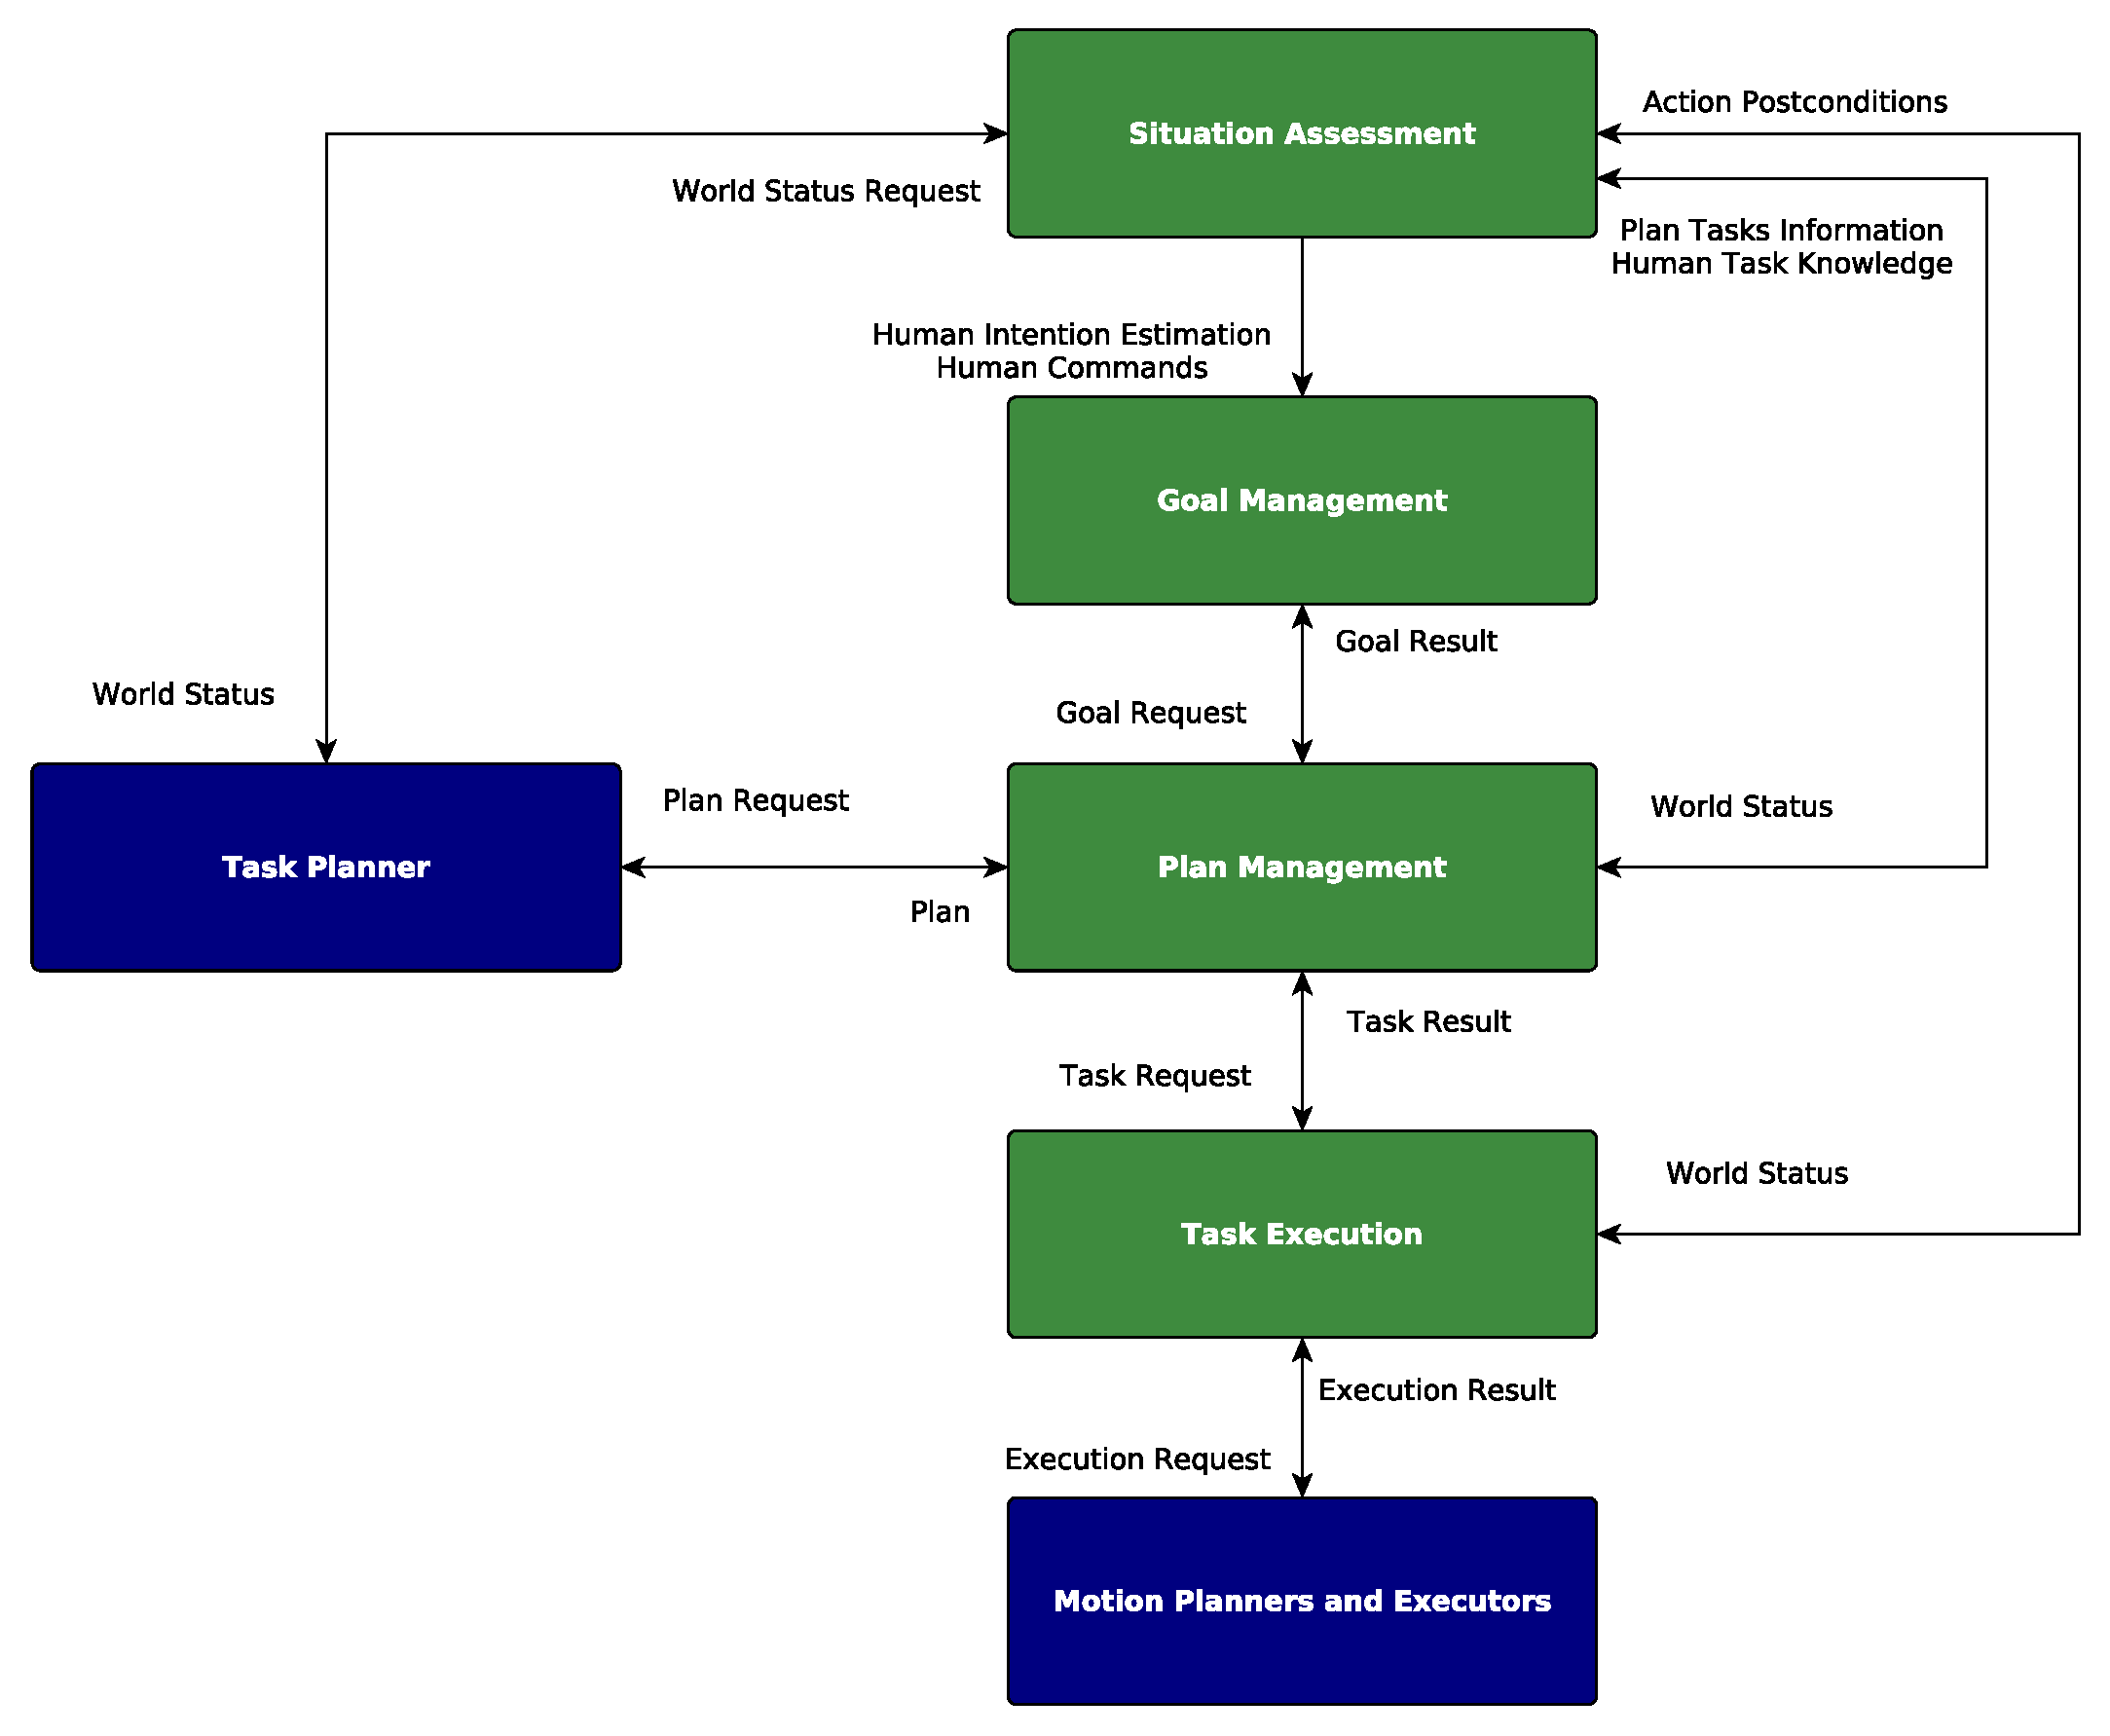
\includegraphics[scale=0.45]{img/intro/system_architecture.pdf}
	\caption[System architecture]{This picture shows the different layers of the system. Green rectangles represent parts of the
	supervision system, while blue rectangles external modules}
	\label{fig:intro-system_architecture}
\end{figure}

The system can also easily interact with different modules, which can be changed depending on the current needs:
\begin{itemize}
\item Task Planner. The Plan Management layer provides an interface for different planners. New planners can be introduced by creating a bridge that respects the interface provided, producing plans in the format requested by the Plan Management layer and reading information about the world state from the Situation Assessment layer.
\item Motion Planners and Executors. The Task Execution layer is interfaced with a set of motion planners and an executor to accomplish the robot's movements and actions. New modules can be introduced by respecting the interface used in the layer.
\end{itemize}


To achieve these goals we use the well-known ROS framework\footnote{http://www.ros.org/}, which naturally supports different robots and modules. The system has been implemented and tested in simulation, using the GAZEBO simulator\footnote{http://gazebosim.org/}, and on two different robots, the PR2 by Willow Garage\footnote{https://www.willowgarage.com/pages/pr2/overview}, and the SPENCER robot\footnote{http://www.spencer.eu/}, developed in an European research project. 

The system has been used in two european projects: SPENCER, whose tasks was building a human-aware robot to guide passengers in an airport scenario; and SAPHARI European project\footnote{http://www.saphari.eu/}, where it was used to execute a cooperative scenario, where a robot and a human had to clean a table together.